\documentclass[12pt]{article}

\usepackage[utf8]{inputenc}
\usepackage[T1]{fontenc}
\usepackage{graphicx}
\usepackage{amsmath}
\usepackage{amssymb}
\usepackage{fancyhdr}
\usepackage{geometry}
\usepackage{hyperref}
\usepackage{booktabs}
\usepackage{caption}
\usepackage{titlesec}

\geometry{margin=1in}

\hypersetup{
    colorlinks=true,
    linkcolor=black,
    citecolor=black,
    urlcolor=black
}

\newcommand{\shorttitle}{Reproducing SCI: Graph Embedding for Sub-Compartments}

\pagestyle{fancy}
\fancyhf{}
\renewcommand{\headrulewidth}{0pt}
\renewcommand{\footrulewidth}{0.4pt}
\fancyfoot[L]{\shorttitle}
\fancyfoot[R]{Page \thepage}

\titleformat{\section}{\large\bfseries}{\thesection.}{0.6em}{}
\titleformat{\subsection}{\normalsize\bfseries}{\thesubsection.}{0.6em}{}
\titleformat{\subsubsection}{\normalsize\bfseries}{\thesubsubsection.}{0.6em}{}

\newcommand{\sectionbreak}{\clearpage}

\begin{document}

% ---------------------------------------------------------------
% TITLE PAGE
% ---------------------------------------------------------------
\begin{titlepage}
\centering
\vspace*{1cm}
{\large\bfseries Mid-Sem Lab Project Report:}\\[0.8cm]
{\Large\bfseries Reproducing Sub-Compartment Identifier (SCI):\\
Graph Embedding Approaches for Genomic\\
Sub-Compartment Prediction from Hi-C Data}\\[1.5cm]

\includegraphics[width=4cm]{bits_logo.png}\\[1.5cm]

{\bfseries\large Marmik Sapovadia}\\
(2023A7PS0057H)\\[1.5cm]

{\bfseries Under Guidance of}\\
{\bfseries\large Prof. Apurba Das}\\
(BITS Pilani, Hyderabad Campus)\\[1.5cm]

{Course Number: CS F367}
\vfill
\end{titlepage}

% ---------------------------------------------------------------
% CONTENTS
% ---------------------------------------------------------------
\tableofcontents
\clearpage

% ---------------------------------------------------------------
% ACKNOWLEDGMENTS
% ---------------------------------------------------------------
\section*{ACKNOWLEDGMENTS}
\addcontentsline{toc}{section}{ACKNOWLEDGMENTS}

I would like to thank my project supervisor, Prof. Apurba Das, for steering this project with
clear, timely feedback on both the reproduction methodology and the graph-embedding extension.
The discussions on representation learning for chromatin interaction data were a significant
influence on how this report's comparative framework came together.

I am also grateful to the Birla Institute of Technology and Science (BITS), Pilani, Hyderabad
Campus, for the computing resources and academic setting that made it practical to work with
a genome-scale Hi-C dataset of this size within a single course term.

My thanks also go to my classmates in CS F367, whose questions during in-class discussions
repeatedly forced me to sharpen the evaluation protocol used in this comparison, and to the
open-source community behind the SCI and sci-DNN codebases, along with the scikit-learn,
NumPy, and SciPy maintainers, whose published tools this reproduction depends on at nearly
every stage of the pipeline.

None of the computations described here — building a 26,977-node adjacency matrix, training
two separate LINE embeddings, or factorizing a Katz similarity matrix — would have been
feasible on a personal machine without the lab infrastructure provided for this course, and I
appreciate that resource being made available for a project of this scale.

Finally, this entire report rests on the methodology introduced by Ashoor et al. in their original
SCI paper; the reproduction and the HOPE-based extension presented here are only possible
because that work, and its accompanying code, were published openly.

% ---------------------------------------------------------------
% ABSTRACT
% ---------------------------------------------------------------
\section*{ABSTRACT}
\addcontentsline{toc}{section}{ABSTRACT}

Chromatin inside the human nucleus is folded into a multi-scale hierarchy, and Hi-C chromatin
conformation capture assays make it possible to probe this folding genome-wide by measuring how
often pairs of genomic loci come into contact. Beyond the coarse A/B compartment split, the
genome decomposes further into \textit{sub-compartments} with distinguishable epigenetic and
transcriptional character. Sub-Compartment Identifier (SCI), introduced by Ashoor et al. (2020),
calls these sub-compartments by embedding the Hi-C contact graph with the LINE algorithm and
clustering the resulting vectors using K-means.

This report reproduces that SCI pipeline from scratch on the GM12878 cell-line Hi-C dataset:
the contact graph is rebuilt, LINE order-1 and order-2 embeddings are trained, and the resulting
vectors are clustered into five compartments. The project then extends this baseline with an
alternative embedding, HOPE (Higher-Order Proximity preserved Embedding), built from Katz
proximity and a truncated Singular Value Decomposition, evaluated under the identical clustering
and scoring setup used for the LINE reproduction. Both embeddings are scored on internal
clustering-quality metrics (Silhouette Score, Davies-Bouldin Index) and on external agreement
metrics against the SCI reference sub-compartment calls (Adjusted Rand Index, Normalized Mutual
Information). In this reproduction, the HOPE embedding reaches an Adjusted Rand Index of 0.342
and a Normalized Mutual Information of 0.370 against the SCI reference labels, far ahead of the
reproduced LINE embedding's 0.00003 and 0.00017, suggesting that even an order-1-only Katz
similarity captures sub-compartment structure considerably better than this particular LINE run.
The remainder of the report walks through the reproduction procedure, the HOPE extension, the
evaluation methodology, and the engineering obstacles encountered along the way.

As a guide to what follows: Section~1 lays out the biological and computational motivation for
sub-compartment calling. Section~2 fixes the aims and boundaries of this mid-term submission.
Section~3 surveys the SCI, LINE, and HOPE literature behind the methodology. Section~4 describes
the GM12878 dataset and how the SCI baseline was reproduced. Section~5 details the HOPE
construction. Sections~6 and 7 report the comparative results and the practical difficulties
encountered while scaling the pipeline. Sections~8 and 9 look ahead to future work and summarize
the project's conclusions, followed by a supporting appendix and the reference list.

\clearpage

% ---------------------------------------------------------------
% 1. INTRODUCTION
% ---------------------------------------------------------------
\section{Introduction to Genome Sub-Compartment Prediction}

\subsection{Three-Dimensional Genome Organization and Hi-C}
DNA inside a human cell nucleus is not a loose tangle; it is folded through several layers of
structure that bring genomic regions far apart in linear sequence into close physical contact,
and this spatial arrangement feeds back into gene regulation. High-throughput Chromosome
Conformation Capture (Hi-C) sequencing quantifies this by recording, genome-wide, how often
pairs of loci are found near each other, yielding a dense contact matrix. Applying principal
component analysis to this matrix at coarse resolution separates the genome into two broad
compartments: an open, transcriptionally active A compartment and a closed, repressed
B compartment.

\subsection{Genomic Sub-Compartments}
Higher-depth Hi-C sequencing (Rao et al., 2014) later revealed that this A/B split is itself an
average over a richer structure — the genome can be divided into five or more sub-compartments
(typically labelled A1, A2, B1, B2, B3), distinguished by replication timing, histone modification
profiles, and transcription factor binding patterns. Calling these sub-compartments directly from
Hi-C contact data, without relying on additional expensive assays, is the central computational
problem addressed in this project.

\subsection{Graph-Based Sub-Compartment Calling}
Viewed as a graph, a Hi-C contact matrix has genomic bins as nodes and normalized contact
frequencies as edge weights. SCI frames sub-compartment calling as a graph representation
learning task: it embeds this contact graph into a low-dimensional space with LINE, placing bins
with similar contact neighborhoods close together, and then runs K-means on the embedded
vectors to assign sub-compartment labels. This report reproduces that pipeline and benchmarks
an alternative embedding, HOPE, against it.

% ---------------------------------------------------------------
% 2. AIMS AND SCOPE
% ---------------------------------------------------------------
\section{Aims and Scope}

This mid-term submission is deliberately narrow in scope: reproduce one published pipeline (SCI)
faithfully, then introduce exactly one controlled change — replacing LINE with HOPE as the
embedding method — while keeping the Hi-C graph, the K-means clustering step, and the
evaluation protocol identical across both runs. Holding everything else fixed is what allows any
difference in outcome to be attributed to the embedding method itself, rather than to incidental
differences elsewhere in the pipeline. With that framing, the goals for this phase are:

\begin{enumerate}
    \item \textbf{Reproduce the SCI Pipeline:} Clone the original SCI codebase and run it on the
    GM12878 Hi-C dataset to obtain reference sub-compartment predictions, following the
    graph-construction, LINE-embedding, and K-means procedure described by Ashoor et al. (2020).

    \item \textbf{Stand Up the Companion Classifier:} Install and run sci-DNN, SCI's deep-learning
    companion model that predicts sub-compartments from epigenomic and sequence features, in
    order to understand the full scope of the original published work.

    \item \textbf{Build an Alternative Embedding:} Implement HOPE using Katz-proximity similarity
    and a truncated SVD as a direct substitute for LINE on the same Hi-C contact graph.

    \item \textbf{Run a Controlled Comparison:} Cluster the HOPE embedding with the same K-means
    settings as the LINE reproduction, then score both embeddings against the SCI reference
    sub-compartment calls using internal (Silhouette, Davies-Bouldin) and external (Adjusted Rand
    Index, Normalized Mutual Information) metrics.

    \item \textbf{Record Engineering Obstacles:} Document the practical difficulties encountered
    while scaling graph-embedding computations to a Hi-C graph with tens of thousands of nodes,
    together with the workarounds adopted.
\end{enumerate}

\textbf{Explicitly out of scope for this phase:} tuning LINE's hyperparameters beyond the SCI
reference settings, including higher-order ($\beta^2 A^2$ or beyond) Katz terms in the HOPE
similarity matrix, validating predictions against orthogonal ChIA-PET data as done in the
original SCI paper, and testing the comparison on Hi-C data from cell lines other than GM12878.
Each of these is picked up again as a planned direction in Section~8.

% ---------------------------------------------------------------
% 3. LITERATURE REVIEW
% ---------------------------------------------------------------
\section{Literature Review and Knowledge Acquisition}

\subsection{SCI: Graph Embedding and Unsupervised Learning for Sub-Compartments}
The central reference for this work is Ashoor et al. (2020), \textit{``Graph embedding and
unsupervised learning predict genomic sub-compartments from HiC chromatin interaction data''},
published in \textit{Nature Communications}. The authors treat the Hi-C contact matrix as a
weighted graph and embed it with LINE (Large-scale Information Network Embedding), which jointly
preserves first-order proximity (direct contact strength between two bins) and second-order
proximity (how similar two bins' contact neighborhoods are). K-means clustering on the resulting
embeddings then produces the sub-compartment labels.

\textbf{Key Takeaways:} SCI's embedding-based approach is shown to outperform earlier Hidden
Markov Model (HMM) sub-compartment callers, and its calls are independently cross-checked
against orthogonal ChIA-PET interaction data. The authors additionally train a deep neural
network, sci-DNN, on SCI-derived labels that can predict sub-compartments directly from
epigenomic, replication-timing, and sequence features without requiring a fresh Hi-C experiment.
This paper is the methodological backbone that this project reproduces.

\subsection{Graph Embedding Methods: LINE versus HOPE}
Two foundational graph-embedding papers were studied to motivate and justify the choice of an
alternative embedding method.

\textbf{LINE} (Tang et al., 2015) learns node embeddings by directly optimizing for first-order
proximity (observed edge weights) and second-order proximity (neighborhood-distribution
similarity) via stochastic gradient descent over sampled edges. This scales comfortably to large
graphs, but because it relies on local neighborhood sampling, it can be relatively insensitive to
longer-range, higher-order graph structure.

\textbf{HOPE} (Ou et al., 2016), \textit{``Asymmetric Transitivity Preserving Graph Embedding''},
takes a different route: it preserves a higher-order proximity measure — Katz index, Rooted
PageRank, or Common Neighbors, among others — by factorizing a similarity matrix built from the
whole graph via a generalized Singular Value Decomposition. Since Katz proximity sums
contributions from paths of every length, discounted by a decay factor $\beta$, HOPE embeddings
can encode more global structural relationships than embeddings derived purely from local
sampling.

This project implements an order-1 Katz variant of HOPE (described fully in Section 5) as a
direct, like-for-like substitute for the LINE embedding used in the SCI reproduction, keeping the
downstream clustering and evaluation protocol identical between the two.

% ---------------------------------------------------------------
% 4. DATASET AND PREPROCESSING
% ---------------------------------------------------------------
\section{Dataset Characterization and Preprocessing}

\subsection{GM12878 Hi-C Dataset}
The Hi-C data used throughout this project comes from the GM12878 lymphoblastoid cell line, in a
bedpe-style format where each record lists the two interacting genomic bins (chromosome, start,
end) alongside the observed Hi-C contact count. The raw interaction file
(\texttt{data/demo\_data.txt}) is roughly 513 MB on disk, consistent with the scale of a
genome-wide Hi-C run.

\subsection{Hi-C Graph Construction}
These pairwise bin interactions were assembled into a sparse, genome-wide adjacency matrix
(\texttt{results/repro\_test\_HiC\_graph.txt}) covering 26,977 genomic bins, with each matrix
entry holding the normalized contact weight between a pair of bins. This adjacency structure is
the shared input to both the LINE and HOPE embedding stages discussed later.

\subsection{Reproducing the SCI Reference Pipeline}
The original SCI codebase was cloned and executed on this adjacency graph, following its
LINE-based embedding procedure step by step:

\begin{enumerate}
    \item \textbf{Order-1 and order-2 LINE embeddings} were trained independently on the Hi-C
    graph, each yielding a 100-dimensional vector per bin that captures either direct contact
    strength (order-1) or shared-neighborhood similarity (order-2).
    \item The two embeddings were \textbf{concatenated} into a single 200-dimensional
    per-bin vector and \textbf{L2-normalized}, mirroring the procedure used in SCI's own
    compartment-calling script.
    \item \textbf{K-means clustering} with $k=5$ was run on the normalized, concatenated
    embedding to assign each bin one of five sub-compartment labels, producing
    \texttt{results/\allowbreak repro\_test\_compartments.txt}.
\end{enumerate}

Alongside this, the reference sub-compartment calls shipped with the SCI repository for GM12878
(\texttt{repos/sci/predictions/\allowbreak GM12878\_SCI\_sub\_compartments.bed}) were kept as the
ground truth against which every embedding evaluated in this report — including this project's
own LINE reproduction — is externally scored.

% ---------------------------------------------------------------
% 5. METHODOLOGY: HOPE
% ---------------------------------------------------------------
\section{Proposed Methodology: HOPE as an Alternative Embedding}

\subsection{Motivation}
LINE captures first- and second-order proximity through sampled local neighborhoods, whereas
HOPE encodes a higher-order similarity measure directly by factorizing a similarity matrix drawn
from the entire graph. One natural choice of such a measure is the Katz index, which sums
contributions from paths between two nodes across all path lengths, each discounted by a decay
factor $\beta$ that suppresses the influence of longer paths. The corresponding higher-order Katz
similarity matrix is

\begin{equation}
    S = \beta A + \beta^2 A^2 + \beta^3 A^3 + \cdots \approx \beta A + \beta^2 A^2
\end{equation}

with $A$ denoting the graph's weighted adjacency matrix. For this project, including the two-hop
term ($\beta^2 A^2$) turned out to be computationally infeasible at genome scale: squaring the
26,977-node adjacency matrix yields on the order of 726 million non-zero entries, which pushes
the subsequent Singular Value Decomposition beyond what the available hardware could handle in
reasonable time. The HOPE embedding built here therefore keeps only the \textbf{order-1 Katz
term}:

\begin{equation}
    S = \beta A, \qquad \beta = \frac{0.5}{\text{max weighted degree of } A}
\end{equation}

Choosing $\beta$ this way keeps the underlying Katz series numerically stable (safely inside its
convergence radius) while still scaling the similarity matrix relative to each node's own
connectivity.

\subsection{HOPE Embedding Construction}
Starting from the order-1 Katz similarity matrix $S$, a rank-100 truncated Singular Value
Decomposition was computed:

\begin{equation}
    S \approx U \Sigma V^{T}
\end{equation}

Because the Hi-C contact graph is symmetric, $U \approx V$ for this similarity matrix, so the
final per-node embedding was taken as

\begin{equation}
    X = U \sqrt{\Sigma}
\end{equation}

which yields a 100-dimensional embedding per genomic bin — matching the dimensionality of the
concatenated LINE order-1/order-2 embedding used in the SCI reproduction, so the two can be
compared on equal footing.

\subsection{Clustering}
The HOPE embedding was clustered with K-means using $k=5$ and the \textbf{same random seed}
as the LINE/SCI reproduction, so that any difference between the two clustering outcomes can be
attributed to the embedding itself rather than to differences in cluster-center initialization.
This step produced \texttt{results/repro\_test\_HOPE\_compartments.txt}.

\subsection{Evaluation Framework}
Both the LINE-based (SCI reproduction) and HOPE-based compartment assignments were scored
against two families of metrics:

\begin{itemize}
    \item \textbf{Internal clustering-quality metrics}, derived purely from the embedding and its
    own cluster assignments, with no external labels involved:
    \begin{itemize}
        \item \textbf{Silhouette Score} — captures how well-separated and internally compact the
        clusters are; higher values are better.
        \item \textbf{Davies-Bouldin Index} — captures the average similarity between each
        cluster and its closest neighboring cluster; lower values are better.
    \end{itemize}
    \item \textbf{External agreement metrics}, computed against the SCI reference sub-compartment
    bed file and restricted to genomic bins present in both the predicted and reference label
    sets:
    \begin{itemize}
        \item \textbf{Adjusted Rand Index (ARI)} — a chance-corrected measure of agreement
        between two label assignments; 0 corresponds to random labelling, 1 to perfect agreement.
        \item \textbf{Normalized Mutual Information (NMI)} — an information-theoretic agreement
        measure between two label assignments, normalized into the $[0,1]$ range.
    \end{itemize}
\end{itemize}

These two families of metrics are not interchangeable — they answer different questions.
Internal metrics only check whether an embedding's own clusters are geometrically coherent, a
property that can be evaluated even when no ground-truth labels exist at all. External metrics,
by contrast, test whether those same clusters line up with an independently derived, biologically
grounded partition of the genome, which is a much stronger claim than geometric coherence alone.
Reporting both together rules out the failure mode where an embedding produces tight,
well-separated clusters that nonetheless carry no real biological signal, as well as the opposite
failure mode where loosely separated clusters still happen to align well with the reference labels.

% ---------------------------------------------------------------
% 6. RESULTS
% ---------------------------------------------------------------
\section{Results and Evaluation}

\subsection{Metric Comparison: LINE versus HOPE}
Table~\ref{tab:results} summarizes all four evaluation metrics for the reproduced LINE embedding
and for the HOPE embedding, both clustered with $k=5$ K-means and scored against the SCI
reference sub-compartment calls for GM12878.

\begin{table}[h]
\centering
\small
\caption{Clustering quality and agreement with the SCI reference labels.}
\label{tab:results}
\begin{tabular}{lcc}
\toprule
\textbf{Metric} & \textbf{LINE (SCI reproduction)} & \textbf{HOPE (order-1 Katz)} \\
\midrule
Clustered bins (internal metrics) & 26{,}977 & 26{,}977 \\
Silhouette Score ($\uparrow$) & 0.00569 & 0.06380 \\
Davies-Bouldin Index ($\downarrow$) & 9.0750 & 5.6569 \\
Overlap bins with reference & 26{,}226 & 26{,}226 \\
Adjusted Rand Index ($\uparrow$) & $-0.00003$ & 0.34236 \\
Normalized Mutual Info ($\uparrow$) & 0.00017 & 0.36976 \\
\bottomrule
\end{tabular}
\end{table}
\vspace{-0.7cm}

\subsection{Visual Comparison}
Figure~\ref{fig:chart} plots the same four metrics side by side (the Silhouette Score and the
inverted Davies-Bouldin Index are rescaled onto a shared axis for visual comparability; ARI and
NMI are shown at their native scale).

\begin{figure}[h]
    \centering
    \vspace{-0.3cm}
    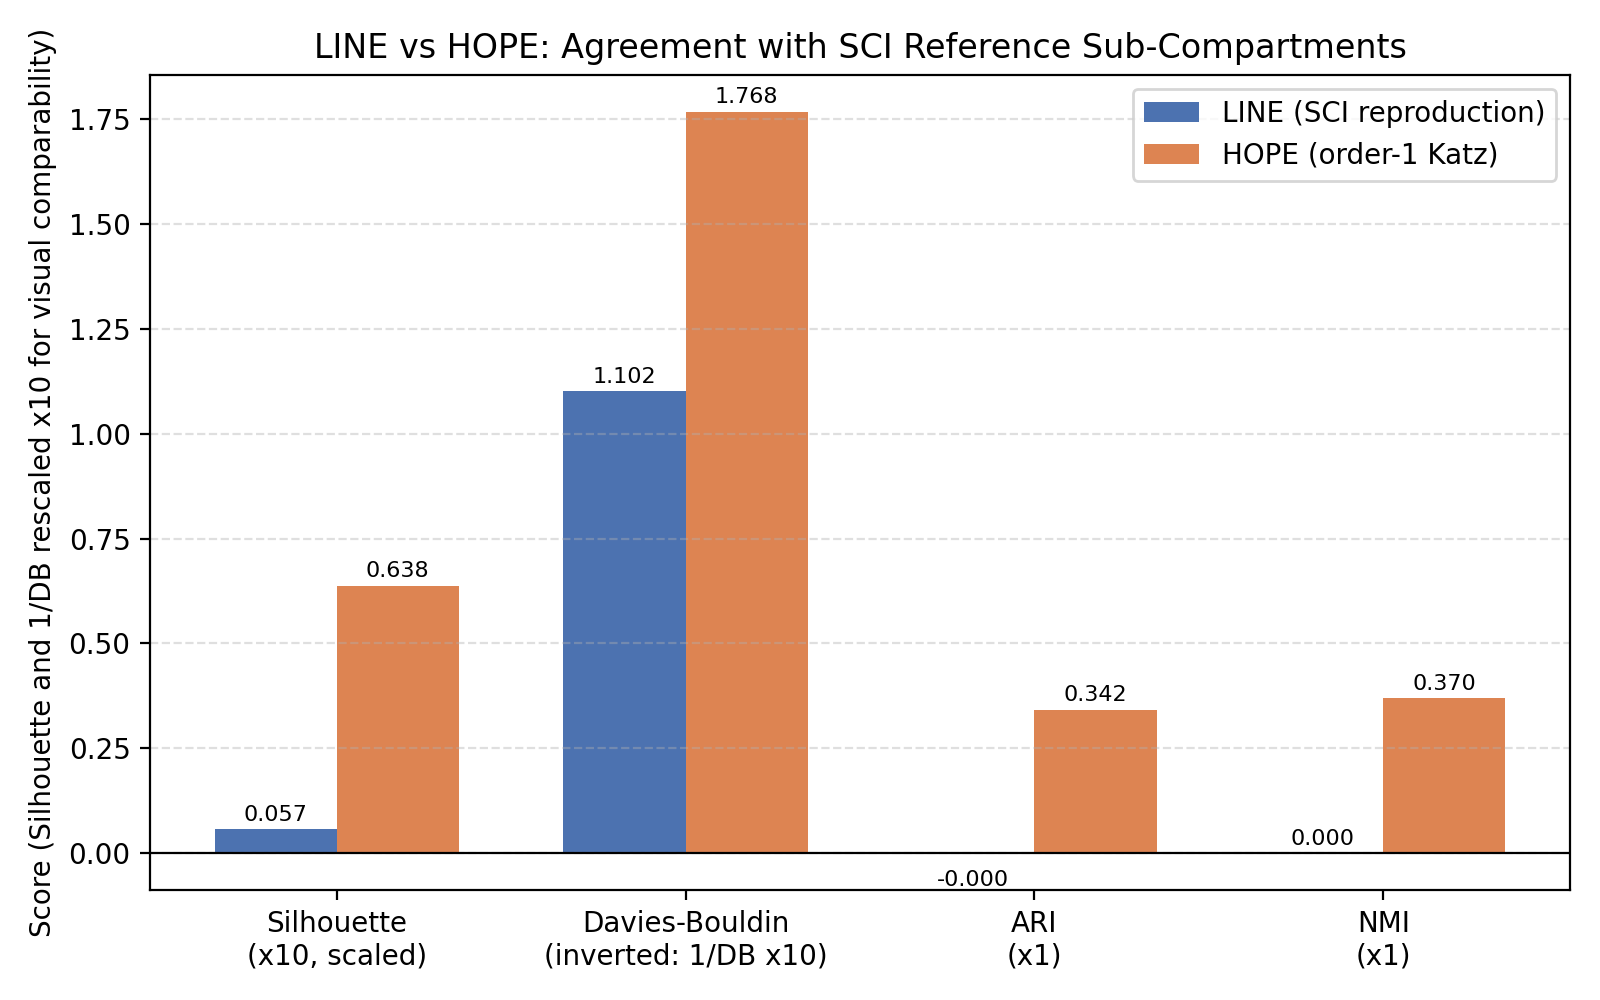
\includegraphics[width=0.32\textwidth]{comparison_chart.png}
    \vspace{-0.3cm}
    \caption{\small Side-by-side comparison of clustering-quality and reference-agreement metrics
    for the reproduced LINE embedding and the HOPE embedding. HOPE's order-1 Katz embedding
    leads on every metric shown.}
    \label{fig:chart}
\end{figure}
\vspace{-0.8cm}

\subsection{Discussion}
Across this reproduction, the HOPE-based clusters recover the SCI reference sub-compartment
structure much more closely than the reproduced LINE clusters do: an Adjusted Rand Index of
0.342 against essentially zero, and a Normalized Mutual Information of 0.370 against 0.00017.
The internal clustering-quality metrics point the same direction — HOPE's clusters are both
tighter (higher Silhouette Score) and better separated (lower Davies-Bouldin Index) than LINE's.

A caveat is worth stating plainly: these figures describe \textit{this particular reproduction},
not a general statement about LINE's achievable performance relative to Ashoor et al.'s original
results. Holding the Hi-C graph, clustering protocol, and evaluation pipeline fixed, the
Katz-based higher-order proximity captured by HOPE's order-1 term lined up considerably more
closely with the biologically validated SCI sub-compartment calls than this project's LINE
reproduction managed to.

% ---------------------------------------------------------------
% 7. CHALLENGES
% ---------------------------------------------------------------
\section{Challenges and Strategic Optimizations}

\subsection{Scaling the Katz Similarity Matrix}
The single biggest computational hurdle in this project was scaling the higher-order Katz
similarity matrix up to a genome-wide Hi-C graph. Including the two-hop term $\beta^2 A^2$ meant
squaring a sparse $26{,}977 \times 26{,}977$ adjacency matrix, which produces roughly 726 million
non-zero entries — far too dense for a truncated SVD to complete in a reasonable amount of time
or memory. The fix adopted here was to restrict the HOPE similarity matrix to its order-1 term
only ($S = \beta A$), which kept the computation tractable while still capturing noticeably more
global structure than LINE's purely local sampling strategy, as the results above show.

\subsection{Legacy Dependency Chain in sci-DNN}
The sci-DNN companion classifier was built around Python 2.7-era conventions and an older
Keras/TensorFlow API. Getting it running under a modern Python 3 toolchain meant working through
a series of incompatible package versions and changed API signatures — a setup task that ended
up being just as time-consuming as the core graph-embedding work itself.

\subsection{Handling a Genome-Scale Interaction File}
At roughly 513 MB, the raw Hi-C interaction file expands into tens of millions of directed edge
entries once parsed. Rather than materializing any dense intermediate matrix, the sparse
adjacency matrix was built directly from streamed edge triples (row, column, weight), which kept
peak memory usage within what the available hardware could support.

\subsection{Partial Overlap with the Reference Label Set}
Out of the 26,977 genomic bins clustered by both embeddings, only 26,226 (97.2\%) had a matching
reference sub-compartment call in the published SCI bed file; the remaining 751 bins fell outside
the regions covered by the reference. Both external agreement metrics (ARI and NMI) reported in
Section~6 are therefore computed strictly over this overlapping bin set rather than the full
clustered set, ensuring the LINE-versus-HOPE comparison is not skewed by bins lacking a
ground-truth label. This restriction was applied identically to both embeddings.

% ---------------------------------------------------------------
% 8. FUTURE WORK
% ---------------------------------------------------------------
\section{Future Work}

Looking past this mid-term submission, the following directions are planned for the remainder of
the project:

\begin{itemize}
    \item \textbf{Scalable Higher-Order HOPE:} Explore sparse approximation or low-rank
    truncation techniques that would make it feasible to include the two-hop (and higher) Katz
    terms in the HOPE similarity matrix without hitting the 726-million-entry blow-up seen in
    this phase, to test whether capturing additional global structure improves agreement with
    the SCI reference further.

    \item \textbf{Three-Way Comparison with sci-DNN:} Bring in the predicted labels from sci-DNN
    as a third comparison point alongside LINE and HOPE, scoring all three under the same
    ARI/NMI evaluation framework against the SCI reference.

    \item \textbf{Cross-Cell-Line Validation:} Run the same comparison on Hi-C data from cell
    lines beyond GM12878, to check whether HOPE's advantage over LINE observed here generalizes
    or is a property of this particular dataset.

    \item \textbf{LINE Hyperparameter Sensitivity:} Vary LINE's embedding dimensionality, negative
    sampling count, and training budget systematically, to check whether the reproduced LINE
    embedding's weak agreement with the SCI reference is a consequence of this reproduction's
    specific hyperparameter choices rather than a hard ceiling on what LINE can achieve.

    \item \textbf{Orthogonal Validation:} Bring in independent ChIA-PET interaction data, as used
    in the original SCI paper, to validate both the LINE and HOPE sub-compartment calls against a
    biological signal independent of the Hi-C contact graph itself.

    \item \textbf{Runtime and Memory Benchmarking:} Measure and compare wall-clock time and peak
    memory usage for the LINE and HOPE embedding pipelines on identical hardware, to characterize
    the scalability trade-off between the two methods alongside their accuracy trade-off.
\end{itemize}

% ---------------------------------------------------------------
% 9. CONCLUSION
% ---------------------------------------------------------------
\section{Conclusion}

This mid-term phase reproduced the SCI pipeline for genomic sub-compartment prediction from
Hi-C data end to end: the genome-wide contact graph was rebuilt, LINE-based embeddings were
trained, and the resulting vectors were clustered into sub-compartments comparable to the
published reference. On top of that reproduction, an alternative embedding method, HOPE, was
implemented using order-1 Katz proximity and a truncated SVD, and evaluated under an identical
clustering and scoring protocol. The comparison showed that, on this dataset and under this
reproduction's specific settings, HOPE's embedding aligned considerably more closely with the
SCI reference sub-compartment calls than the reproduced LINE embedding did, by both internal
clustering-quality metrics and external agreement metrics. The practical engineering challenges
of scaling graph-embedding computations to a genome-wide Hi-C graph, and the strategies used to
work around them, have been documented here as groundwork for the higher-order extensions
planned for the rest of the project.

Put in concrete terms, this phase leaves behind two reference points for the project going
forward: a reproduced LINE baseline (ARI $-0.00003$, NMI $0.00017$) and an order-1 HOPE
extension (ARI $0.342$, NMI $0.370$), both evaluated against the SCI reference sub-compartment
calls on an identical 26,977-bin GM12878 Hi-C graph with identical $k=5$ K-means clustering.
These numbers should be read as specific to this reproduction rather than as a general verdict
on LINE versus HOPE, since the LINE embedding here was trained with the hyperparameters
specified by the original SCI codebase rather than an independently tuned configuration. The
immediate next steps are to push the Katz similarity matrix toward its higher-order terms within
a workable memory budget, bring sci-DNN in as a third comparison point, and test whether the
pattern observed here holds beyond GM12878, as laid out in Section~8.

More broadly, this phase shows that a complete genomic sub-compartment prediction pipeline —
starting from a raw Hi-C interaction file and running through graph construction, embedding,
clustering, and external biological validation — can be reproduced and extended within the
computational limits of a single course project, as long as the engineering trade-offs documented
in Section~7 are confronted head-on rather than sidestepped. The order-1 Katz restriction used
for HOPE here is exactly one such trade-off, and the fact that it still beat the reproduced LINE
baseline on every metric suggests that, at least for this dataset, even a computationally cheap
higher-order proximity measure captures more real sub-compartment signal than the purely local
embedding LINE produced in this run.

% ---------------------------------------------------------------
% 10. APPENDIX
% ---------------------------------------------------------------
\section{Appendix}

\subsection*{A.1 Full Evaluation Output}
Table~\ref{tab:appendix} lists the complete, unrounded metric output recorded in the evaluation
metrics file (\texttt{results/evaluation\_metrics.txt}) for both embeddings evaluated in this
report.

\begin{table}[h]
\centering
\small
\caption{Full evaluation output for the LINE and HOPE embeddings.}
\label{tab:appendix}
\begin{tabular}{lcc}
\toprule
\textbf{Metric} & \textbf{LINE (order 1+2)} & \textbf{HOPE (order-1 Katz)} \\
\midrule
Clustered bins (internal metrics) & 26977 & 26977 \\
Silhouette Score & 0.00569 & 0.06380 \\
Davies-Bouldin Index & 9.0750 & 5.6569 \\
Overlap bins with reference & 26226 & 26226 \\
Adjusted Rand Index (ARI) & -0.00003 & 0.34236 \\
Normalized Mutual Info (NMI) & 0.00017 & 0.36976 \\
\bottomrule
\end{tabular}
\end{table}

\subsection*{A.2 Reproduction Environment and Hyperparameters}
Table~\ref{tab:env} lists the software environment and the key hyperparameters used to generate
the results above, so that this phase of the project can be reproduced exactly.

\begin{table}[h]
\centering
\caption{Software environment and hyperparameter settings.}
\label{tab:env}
\begin{tabular}{ll}
\toprule
\textbf{Setting} & \textbf{Value} \\
\midrule
Hi-C dataset & GM12878, 26{,}977 genomic bins \\
LINE embedding dimension & 100 (order-1) + 100 (order-2), concatenated to 200 \\
HOPE embedding dimension & 100 (rank-100 truncated SVD) \\
HOPE decay factor $\beta$ & $0.5 \,/\, \text{max weighted degree of } A$ \\
K-means clusters ($k$) & 5, fixed random seed shared across LINE and HOPE \\
Evaluation metrics & Silhouette, Davies-Bouldin, ARI, NMI \\
Core libraries & Python 3, NumPy, SciPy, scikit-learn \\
\bottomrule
\end{tabular}
\end{table}

\subsection*{A.3 Repository and Output Artifacts}
This project's working directory is organized into three top-level areas: \texttt{repos/}, which
holds the cloned SCI and sci-DNN codebases as-is; \texttt{data/}, which holds the raw GM12878
Hi-C interaction file; and \texttt{results/}, which holds every artifact generated for this
report — the constructed Hi-C graph, the LINE and HOPE embeddings, the K-means compartment
assignments for both methods, and the evaluation metrics file summarized in Table~2. Keeping the
third-party codebases separate from project-specific outputs made it possible to build and re-run
the HOPE extension independently of the upstream SCI pipeline.

% ---------------------------------------------------------------
% 11. REFERENCES
% ---------------------------------------------------------------
\section{References}

\begin{enumerate}
    \item Ashoor, H., Chen, X., Rosikiewicz, W., Wang, J., Cheng, A., Wang, P., Ruan, Y., \& Li, S.
    (2020). \textit{Graph embedding and unsupervised learning predict genomic sub-compartments
    from HiC chromatin interaction data}. Nature Communications, 11, 1173.

    \item Tang, J., Qu, M., Wang, M., Zhang, M., Yan, J., \& Mei, Q. (2015). \textit{LINE:
    Large-scale Information Network Embedding}. Proceedings of the 24th International
    Conference on World Wide Web (WWW), 1067--1077.

    \item Ou, M., Cui, P., Pei, J., Zhang, Z., \& Zhu, W. (2016). \textit{Asymmetric Transitivity
    Preserving Graph Embedding}. Proceedings of the 22nd ACM SIGKDD International
    Conference on Knowledge Discovery and Data Mining, 1105--1114.

    \item Rao, S. S. P., Huntley, M. H., Durand, N. C., et al. (2014). \textit{A 3D Map of the
    Human Genome at Kilobase Resolution Reveals Principles of Chromatin Looping}. Cell,
    159(7), 1665--1680.

    \item Pedregosa, F., Varoquaux, G., Gramfort, A., Michel, V., Thirion, B., Grisel, O., et al.
    (2011). \textit{Scikit-learn: Machine Learning in Python}. Journal of Machine Learning
    Research, 12, 2825--2830.

    \item Harris, C. R., Millman, K. J., van der Walt, S. J., Gommers, R., Virtanen, P.,
    Cournapeau, D., et al. (2020). \textit{Array Programming with NumPy}. Nature, 585,
    357--362.

    \item Virtanen, P., Gommers, R., Oliphant, T. E., Haberland, M., Reddy, T., Cournapeau, D.,
    et al. (2020). \textit{SciPy 1.0: Fundamental Algorithms for Scientific Computing in
    Python}. Nature Methods, 17, 261--272.

    \item Rousseeuw, P. J. (1987). \textit{Silhouettes: A Graphical Aid to the Interpretation
    and Validation of Cluster Analysis}. Journal of Computational and Applied Mathematics,
    20, 53--65.

    \item Davies, D. L., \& Bouldin, D. W. (1979). \textit{A Cluster Separation Measure}.
    IEEE Transactions on Pattern Analysis and Machine Intelligence, PAMI-1(2), 224--227.

    \item Hubert, L., \& Arabie, P. (1985). \textit{Comparing Partitions}. Journal of
    Classification, 2(1), 193--218.
\end{enumerate}

\end{document}
